\chapter{Visualização e Análise de Dados}

\section{Visualização centralizada no Grafana}

A visualização dos dados de telemetria assume um papel crucial para a compreensão e monitorização eficaz de sistemas distribuídos. Embora as ferramentas Prometheus, Jaeger e Loki disponham de interfaces próprias para análise independente de métricas, traces e logs, a fragmentação das informações pode dificultar a correlação rápida entre estes dados. Por esse motivo, optou-se pelo Grafana como camada de visualização unificada, visando uma experiência integrada e eficiente.

Entre as principais vantagens destacam-se:

\begin{itemize}
    \item Centralização das métricas, logs e traces num único painel interativo;
    \item Capacidade avançada de correlação entre diferentes tipos de dados, facilitando a identificação de causas-raiz nas anomalias;
    \item Configuração unificada de alertas que abrange todas as fontes de dados;
    \item Interface intuitiva e personalizável, acessível para diversos perfis técnicos;
    \item Linguagens de consulta especializadas (PromQL, LogQL) diretamente integradas.
\end{itemize}

Assim, o Grafana habilita uma abordagem de "single pane of glass", essencial para o acompanhamento consolidado do desempenho e saúde do sistema e traces de chamadas entre serviços, com visualização temporal.

\break

\section{Organização dos Dashboards}

Os dashboards no Grafana foram estruturados em três categorias principais:

\begin{itemize}
    \item \textbf{Métricas da Aplicação}: monitorização do número de requisições HTTP por segundo, latência média e percentis (p95 e p99), taxas de erro 4xx e 5xx, além do uso de memória da aplicação \texttt{.NET};
    \item \textbf{Infraestrutura Kubernetes}: dados provenientes do Node Exporter relativos à utilização de CPU por nó e pod, carga do sistema (load average), e espaço de disco e memória física utilizados;
    \item \textbf{Logs e Traces}: visualização de logs estruturados filtrados por nível, mensagem e nome do serviço, análise de spans por rota, duração e código de estado, bem como visualização temporal das chamadas entre serviços através dos traces.
\end{itemize}

Esta organização aprimora a navegação e facilita a análise rápida e contextualizada.

\subsection{Paineis e Dashboards}

Para efeito de apresentação e análise, os dashboards apresentados neste capítulo focam-se exclusivamente nos dados relativos ao serviço específico TicketsManagement. Embora fosse perfeitamente possível incluir visualizações de outros ser-viços da arquitetura, tal abordagem tenderia a revelar informações redundantes, uma vez que os padrões e métricas observados seriam semelhantemente aplicáveis. Assim, esta escolha visa proporcionar uma análise mais clara e exemplar, evitando a dispersão do foco e privilegiando a profundidade sobre a generalidade.

\begin{figure}[H]
    \centering
    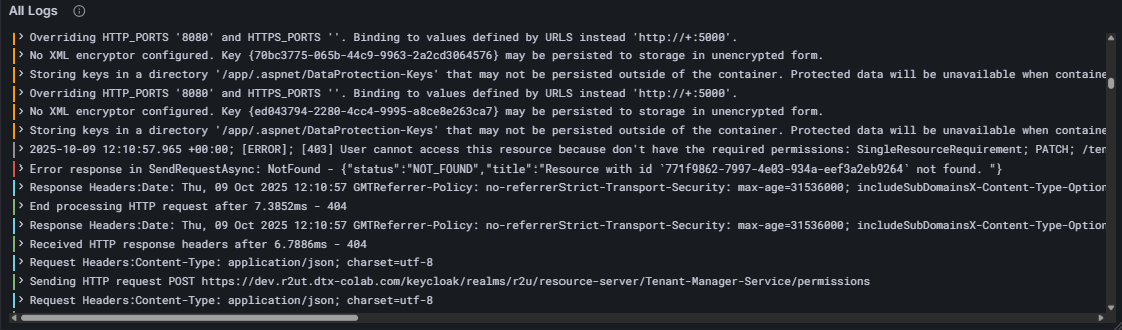
\includegraphics[width=1\textwidth]{images/Grafana/all_logs_dashboard.png}
    \caption{Painel global de Logs}
    % \label{fig:digital_twin}
\end{figure}

\begin{figure}[H]
    \centering
    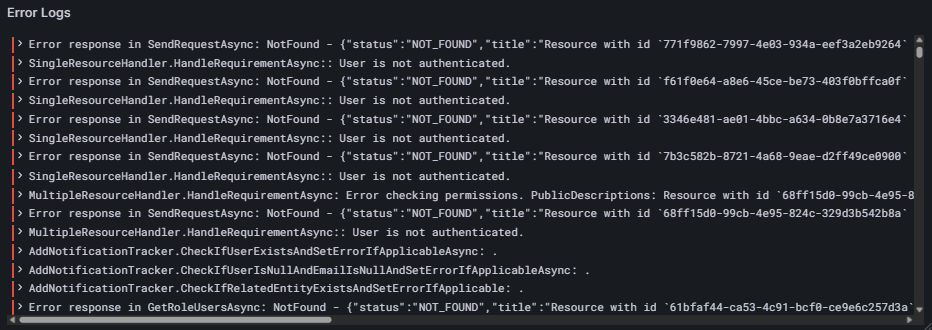
\includegraphics[width=1\textwidth]{images/Grafana/error_logs_dashboard.png}
    \caption{Painel de Logs de Erro}
    % \label{fig:digital_twin}
\end{figure}

\begin{figure}[H]
    \centering
    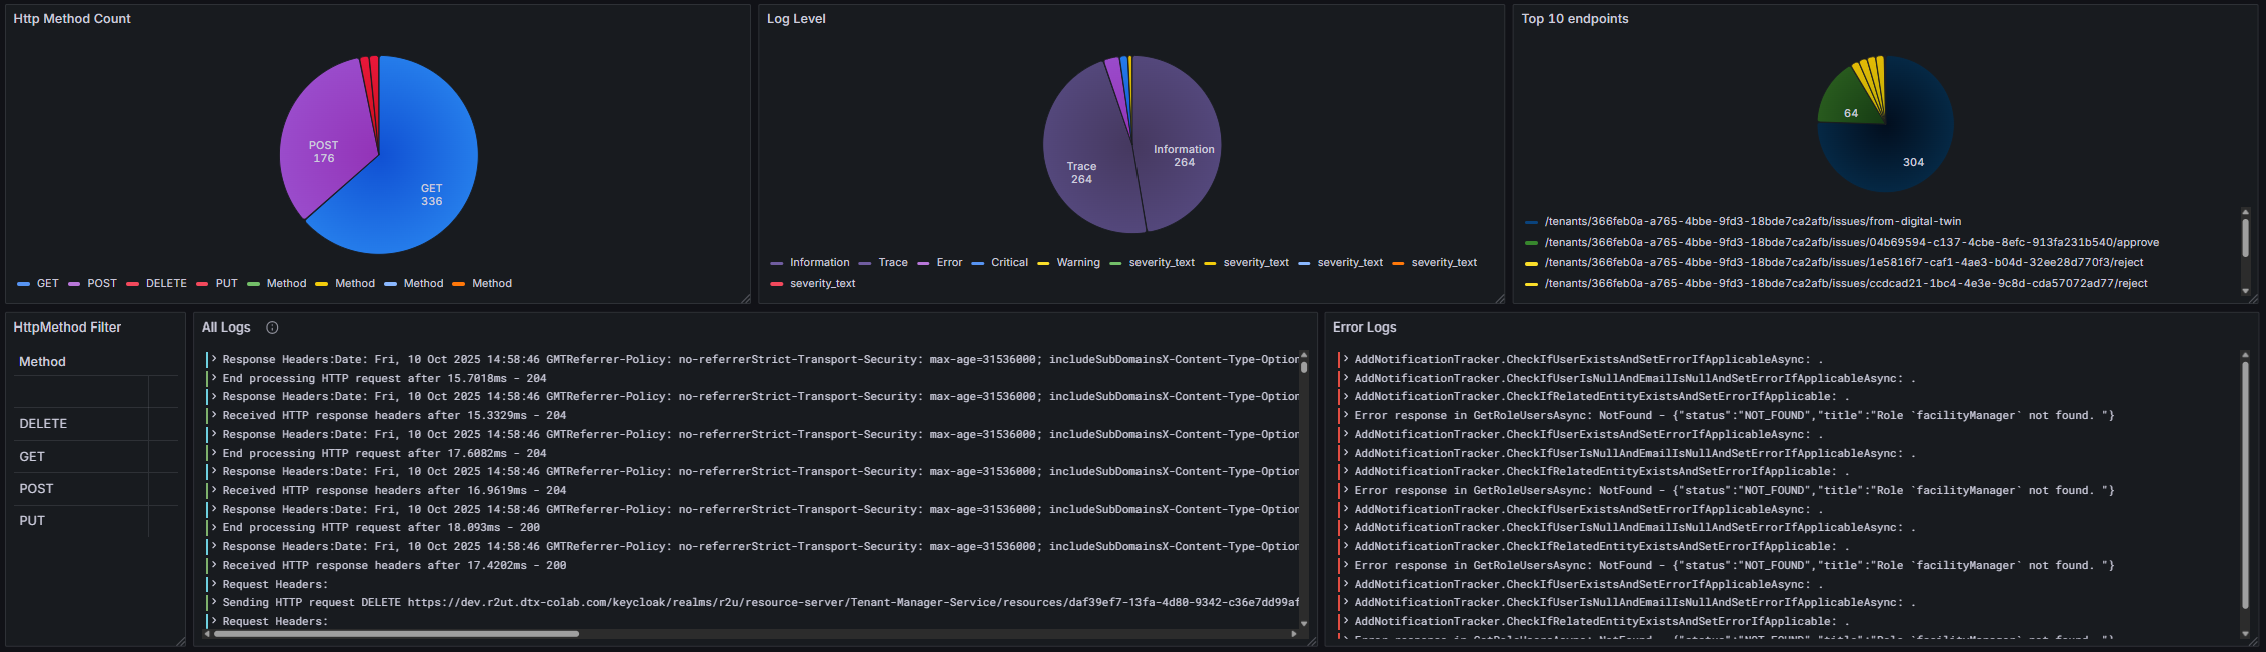
\includegraphics[width=1\textwidth]{images/Grafana/dashboard.png}
    \caption{\textit{Dashboard} de \textit{Logs}}
    % \label{fig:digital_twin}
\end{figure}

\begin{figure}[H]
    \centering
    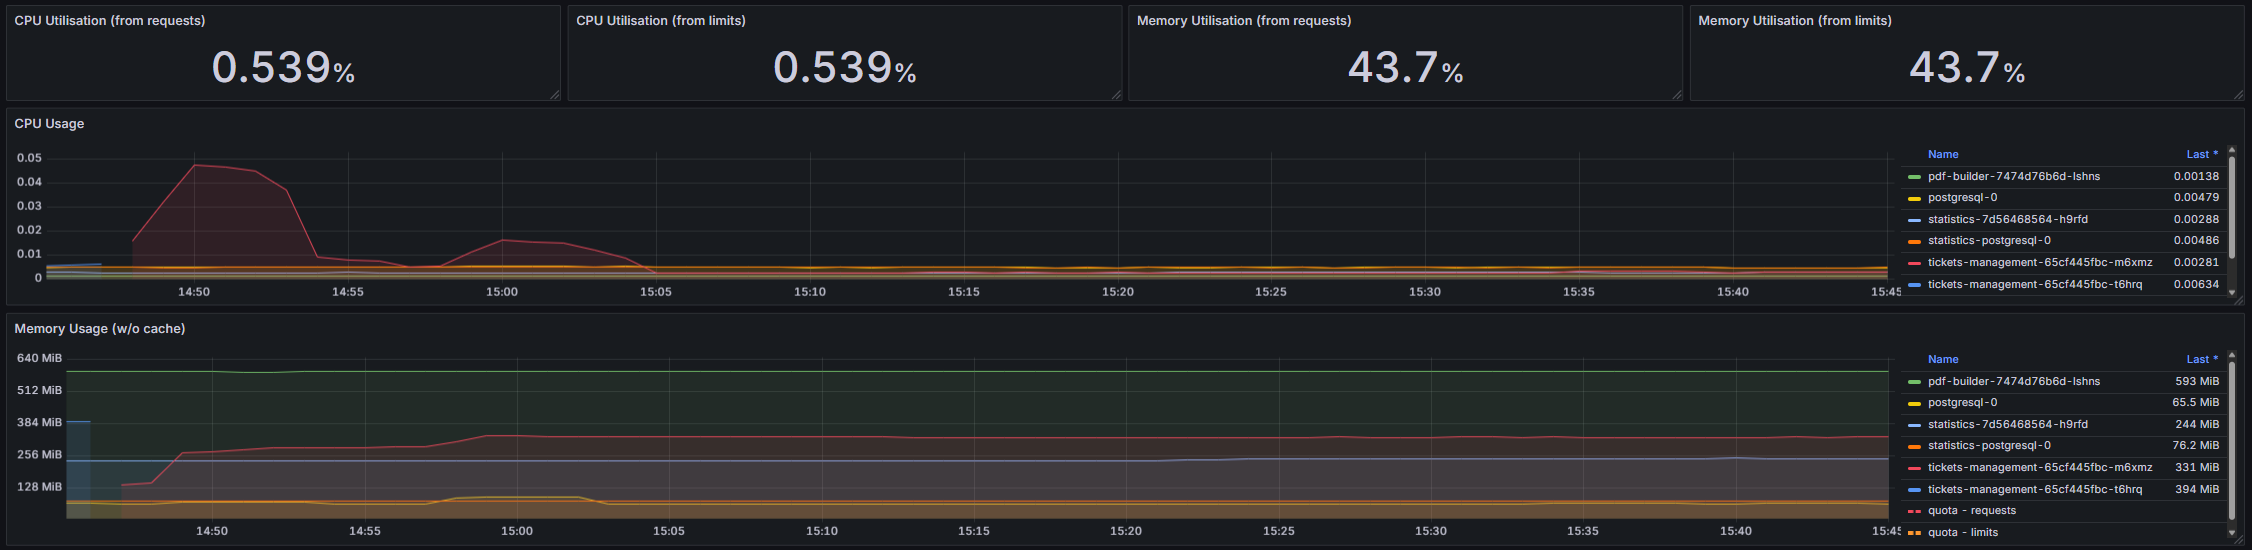
\includegraphics[width=1\textwidth]{images/Grafana/cpu_memory_dashboard.png}
    \caption{Uso de CPU e Memória}
    % \label{fig:digital_twin}
\end{figure}

\begin{figure}[H]
    \centering
    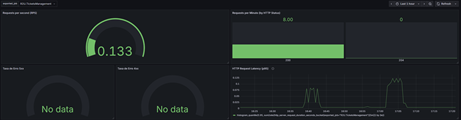
\includegraphics[width=1\textwidth]{images/Grafana/metrics_dashboard.png}
    \caption{Dashboard de metricas: p95, Taxa de Erro, Pedidos por segundo}
    % \label{fig:digital_twin}
\end{figure}

\section{Correlação entre Logs e Traces}

Um dos principais ganhos trazidos pelo Grafana é a correlação direta entre logs e traces. Com um dashboard dedicado, foi possível implementar múltiplos filtros, incluindo o \texttt{service\_name}, que permitem visualizar os logs emitidos por diferentes serviços e vinculá-los diretamente às requisições (traces) correspondentes que os originaram.

Cada entrada de log disponibiliza um link direto para o trace associado, simplificando significativamente a depuração e o diagnóstico de problemas. Este recurso proporciona uma visão holística do estado do sistema e das suas interações, facilitando a identificação rápida de causas de falhas ou degradação do serviço.

\begin{figure}[H]
    \centering
    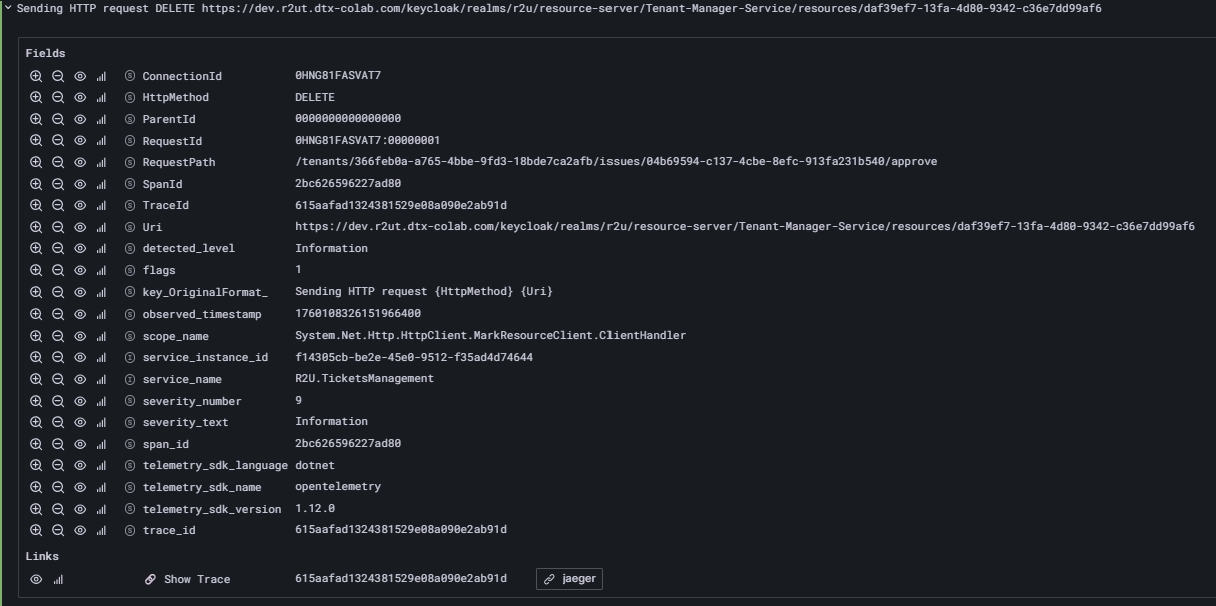
\includegraphics[width=1\textwidth]{images/Grafana/log_expanded.png}
    \caption{Log: Correlação Log e Trace}
    % \label{fig:digital_twin}
\end{figure}

\begin{figure}[H]
    \centering
    
\includegraphics[width=1\textwidth]{images/Grafana/trace link por log.png}
    \caption{Link para Trace}
    % \label{fig:digital_twin}
\end{figure}

\begin{figure}[h]
    \centering
    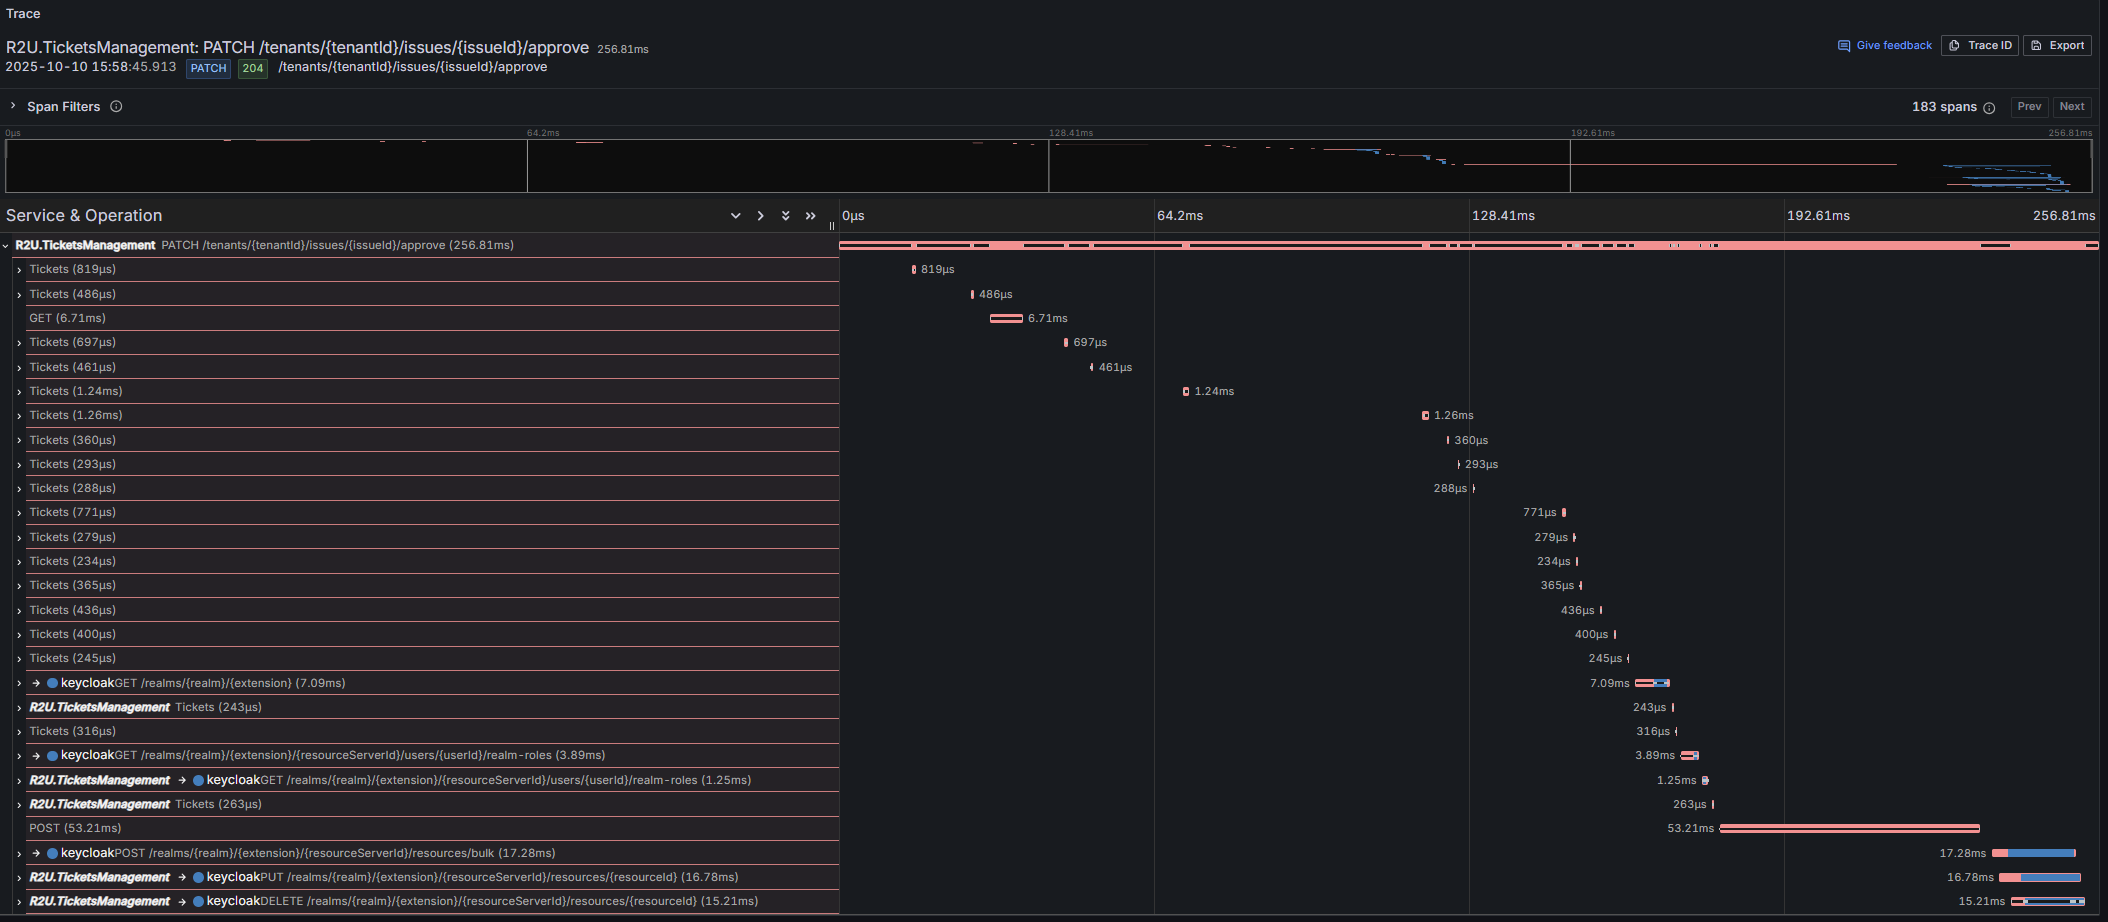
\includegraphics[width=1\textwidth]{images/Grafana/trace_approve.png}
    \caption{Trace: Correlação Log e Trace}
    % \label{fig:digital_twin}
\end{figure}

\section{Alertas}

todo: falar um pouco sobre os alertas, ainda nao implementados, mas de configuracao muito simples